\section{Through-going Pion}
\label{Sec:Pion}
\begin{itemize}
\item Explain Landau distribution ("bare" track and "dressed" track)
\item pion track (800 MeV/c) and soft electron ($\sim$10 keV) has different $dE/dx$ = recombination
\item Set delta-ray cut off = 10 keV in simulation, and take ICARUS measurement of recombination.
\item Hit charge distribution is in good agreement between data and MC.
\end{itemize}

\begin{figure}[htbp]
 \begin{center}
  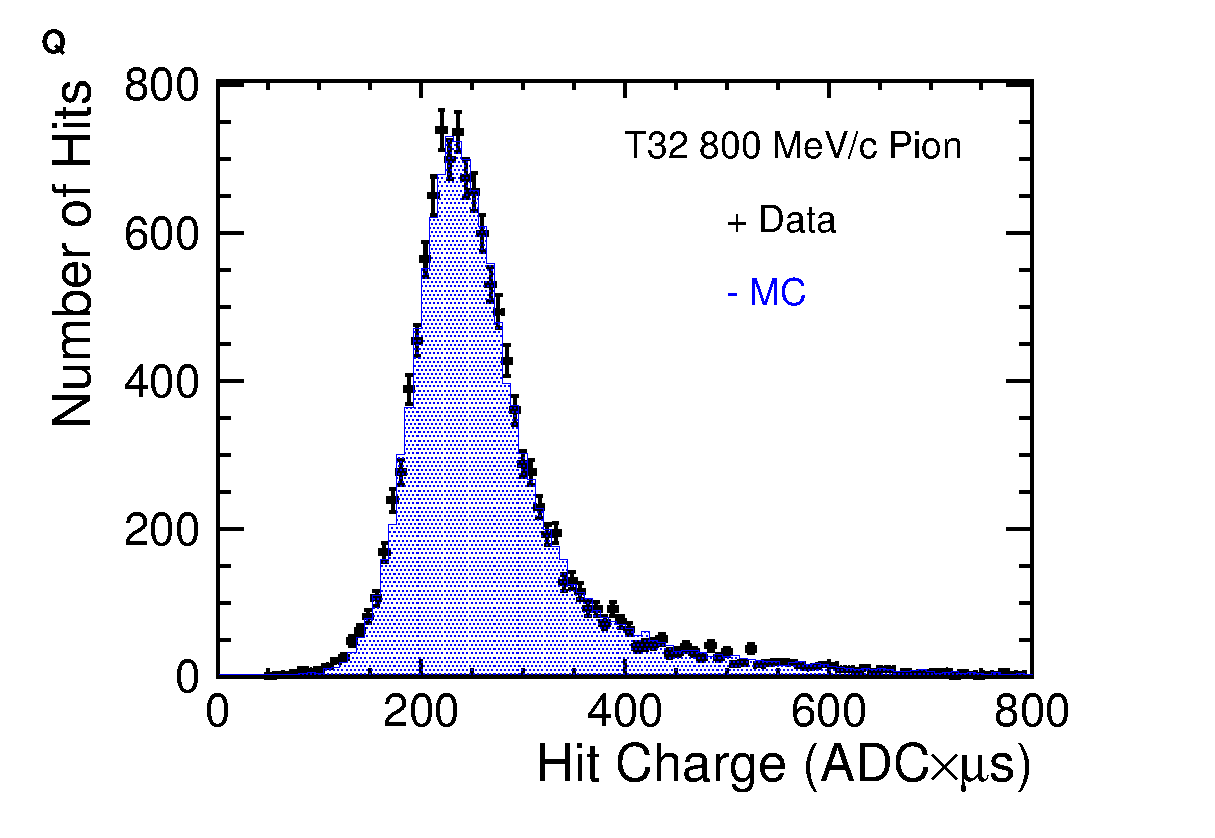
\includegraphics[width=0.8\hsize]{fig/PionLandau.eps}
 \end{center}
 \caption{Hit charge distribution for 800 MeV/c through-going $\pi^+$ sample. Points and histograms correspond to data and MC, respectively}
 \label{Fig:PionLandau}
\end{figure}
